\documentclass[aspectratio=169, 11pt]{beamer}
% ============================================================================
%  23CSE498 -- Project Phase 2, Panel Review 1
%  Structural Descriptors for Metal-Organic Frameworks
%  Compile:  pdflatex panel_review.tex   (twice, for the section numbering)
%  Note: \bibliography is commented out -- references are typeset directly so
%        the deck compiles without needing a bibtex pass. Uncomment if wanted.
% ============================================================================
\usepackage[utf8]{inputenc}
\usepackage[T1]{fontenc}
\usepackage{xcolor}
\usepackage{booktabs}
\usepackage{graphicx}
\usepackage{amsmath}
\usepackage{tikz}
\usetikzlibrary{calc, arrows.meta, positioning}
\graphicspath{{../}{./}{../4_reference/}}
\IfFileExists{opensans.sty}{\usepackage[default,scale=0.95]{opensans}}{}

% --- Branding ---
\definecolor{amritaMaroon}{HTML}{A4123F}
\definecolor{okGreen}{HTML}{0D6B47}
\definecolor{warnRed}{HTML}{B02A2A}
\definecolor{coolBlue}{HTML}{1F5FA8}
\definecolor{softGrey}{HTML}{F4F6FA}

\usetheme{Madrid}
\usecolortheme[named=amritaMaroon]{structure}
\setbeamertemplate{navigation symbols}{}
\setbeamertemplate{footline}[frame number]
\setbeamertemplate{itemize items}[circle]
\setbeamerfont{block title}{size=\small}

\begin{document}

% ============================ TITLE ==========================================
\begin{frame}
    \begin{tikzpicture}[remember picture,overlay]
        \node[fill=amritaMaroon, text=white, font=\bfseries\footnotesize,
              anchor=north east, rounded corners=2pt, inner sep=5pt]
        at ($(current page.north east) + (-0.2cm,-0.2cm)$)
        {Type 1: Research Project};
    \end{tikzpicture}
    \centering
    \IfFileExists{logo.png}{\includegraphics[width=2.4cm]{logo.png}}{\vspace{1.2cm}}
    \vspace{0.05cm}

    {\large \textbf{\textcolor{amritaMaroon}{Structural Descriptors for Metal--Organic
    Frameworks:}}}\\
    {\normalsize \textbf{\textcolor{amritaMaroon}{Multifractal Analysis of Framework
    Connectivity for Simulation-Free Screening}}} \\
    \vspace{0.05cm}
    {\footnotesize \textbf{23CSE498 -- Project Phase 2 (Panel Review 1)} \quad | \quad
     \textbf{Team Number: [XX]}} \\
    \vspace{0.1cm}

    \begin{table}
        \centering
        \scriptsize
        \renewcommand{\arraystretch}{1.05}
        \begin{tabular}{|c|c|l|}
            \hline
            \textbf{S.No} & \textbf{Register Number} & \textbf{Student Name} \\
            \hline
            1 & CB.SC.U4CSE23134 & P. M. Radha Krishna \\
            \hline
            2 & CB.SC.U4CSE23122 & P. Kshitij Varma \\
            \hline
            3 & CB.SC.U4CSE23141 & G. Rohith Abhinav \\
            \hline
            4 & CB.SC.U4CSE23031 & J. Keerthi Sree \\
            \hline
            5 & CB.SC.U4CSE23029 & Isha Sri Prakash \\
            \hline
        \end{tabular}
    \end{table}
    \vspace{0.05cm}

    {\footnotesize Guide: \textbf{Dr.~T.~Ramraj}, M.E, Ph.D --- Assistant Professor (Sl.\,Gd.),}\\
    {\footnotesize Department of Computer Science and Engineering, School of Computing, Coimbatore} \\
    \vspace{0.05cm}
    {\scriptsize \today}
\end{frame}

% ============================ PROBLEM CONTEXT ================================
\section{Problem Context}
\begin{frame}{0. Problem Context --- Why This Project Exists}
\framesubtitle{The gap between the number of candidate materials and our ability to evaluate them}
\begin{columns}[T]
\column{0.54\textwidth}
\textbf{The materials-science problem}
\begin{itemize}\footnotesize
  \item \textbf{Metal--organic frameworks (MOFs)} are crystalline solids built by joining
        metal clusters (\textit{nodes}) to organic molecules (\textit{linkers}).
  \item They are extremely porous --- internal surface areas above
        3{,}000\,m$^2$/g --- making them candidates for gas storage, carbon capture and
        separation.
  \item \textbf{Hundreds of thousands} of MOFs are known or hypothesised.
\end{itemize}

\vspace{0.15cm}
\textbf{The computational bottleneck}
\begin{itemize}\footnotesize
  \item Evaluating one MOF by molecular simulation (GCMC) takes \textbf{hours}.
  \item Exhaustive screening of the design space is \textbf{not feasible}.
\end{itemize}

\column{0.46\textwidth}
\begin{block}{\footnotesize Research Question}
\footnotesize
Can a \textbf{purely structural, simulation-free descriptor} --- computed from a framework's
\textit{connectivity} in seconds --- group MOFs into meaningful families, so a new candidate
can be triaged \textbf{without} expensive calculation?
\end{block}

\vspace{0.1cm}
\begin{block}{\footnotesize Value Proposition}
\footnotesize
Not a \textit{replacement} for simulation --- a \textbf{filter} that decides
\textbf{what to simulate}. Reducing $10^5$ candidates to $10^2$ is the contribution.
\end{block}
\end{columns}
\end{frame}

% ============================ SLIDE 1: METHODOLOGY ===========================
\section{Methodology \& Solution Design}
\begin{frame}{1. Methodology \& Solution Design}
\framesubtitle{Rubric: Workflow, Architecture, Algorithms/Mathematical Model \& Evaluation Metrics (5 Marks)}
\begin{columns}[T]
\column{0.46\textwidth}
{\scriptsize
\textbf{Theoretical foundation.} A MOF is a \textbf{periodic graph}. Collapse each building
block to a vertex and each inter-block bond to an edge; the chemistry reduces to pure
connectivity, which the properties follow.

\vspace{0.12cm}
\textbf{Core algorithms}
\begin{itemize}\scriptsize
  \item \textbf{Decomposition:} MOFid metal-oxo algorithm~[1] --- PBC-aware bond
        perception, connected-component block extraction.
  \item \textbf{Graph construction:} \textit{labelled quotient graph} --- edges carry a
        lattice translation $t$, so the infinite crystal is represented exactly.
  \item \textbf{Descriptor:} influential-node multifractal analysis (iNMFA)~[2].
\end{itemize}

\vspace{0.12cm}
\textbf{Dataset.} \textbf{138 frameworks}: 77 hypothetical (hMOF, via MOFX-DB~[7]) and 61
experimentally synthesised (CoRE MOF 2019, via its Zenodo DOI), both with published PLD/LCD
pore diameters. Supercells of 1{,}160--7{,}000 atoms.
}

\column{0.54\textwidth}
\centering
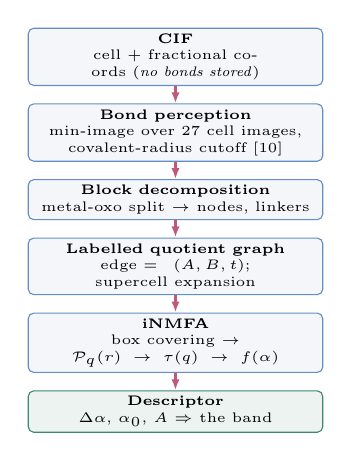
\begin{tikzpicture}[
  node distance=0.22cm,
  every node/.style={font=\tiny},
  box/.style={draw=coolBlue!70, fill=softGrey, rounded corners=2pt,
              text width=3.6cm, align=center, inner sep=2pt, minimum height=0.40cm},
  outbox/.style={draw=okGreen!80, fill=okGreen!8, rounded corners=2pt,
              text width=3.6cm, align=center, inner sep=2pt, minimum height=0.40cm},
  ar/.style={-{Latex[length=1.4mm]}, draw=amritaMaroon!70, thick}]
  \node[box] (a) {\textbf{CIF} \\ cell + fractional coords (\textit{no bonds stored})};
  \node[box, below=of a] (b) {\textbf{Bond perception} \\ min-image over 27 cell images,
                              covalent-radius cutoff~[10]};
  \node[box, below=of b] (c) {\textbf{Block decomposition} \\ metal-oxo split $\to$ nodes,
                              linkers};
  \node[box, below=of c] (d) {\textbf{Labelled quotient graph} \\ edge $=(A,B,t)$;
                              supercell expansion};
  \node[box, below=of d] (e) {\textbf{iNMFA} \\ box covering $\to \mathcal{P}_q(r) \to
                              \tau(q) \to f(\alpha)$};
  \node[outbox, below=of e] (f) {\textbf{Descriptor} \\ $\Delta\alpha$, $\alpha_0$, $A$
                                 $\Rightarrow$ the band};
  \draw[ar] (a)--(b); \draw[ar] (b)--(c); \draw[ar] (c)--(d);
  \draw[ar] (d)--(e); \draw[ar] (e)--(f);
\end{tikzpicture}

\vspace{0.05cm}
{\tiny \textbf{Validation metric:} published \textbf{coordination numbers} --- an
independent ground truth the graph must reproduce.}
\end{columns}
\end{frame}

% ============================ SLIDE 1b: MATH =================================
\begin{frame}{1b. Mathematical Model}
\framesubtitle{The descriptor, defined}
\begin{center}
\begin{minipage}{0.68\textwidth}
\footnotesize
\setlength{\abovedisplayskip}{3pt}
\setlength{\belowdisplayskip}{3pt}
\setlength{\abovedisplayshortskip}{2pt}
\setlength{\belowdisplayshortskip}{2pt}

\textbf{Step 1 --- the measure.} For each influential node $i$ (top 20\% by degree) and box
radius $r$ (a \textbf{graph} quantity, counted in hops between blocks --- not to be confused
with a physical pore diameter in \AA), let $M_i(r)$ be the number of vertices within $r$
steps:
\[ p_i(r) = M_i(r)/N \]

\textbf{Step 2 --- the partition function}, reweighted by a distortion factor $q$:
\[ \mathcal{P}_q(r) = \sum_{i \in I} p_i(r)^{\,q} \]

\textbf{Step 3 --- the mass exponent}, fitted through the origin:
\[ \boxed{\ \tau(q) = \frac{\ln \mathcal{P}_q(r)}{\ln (r/r_N)}\ } \]

\textbf{Step 4 --- Legendre transform.}
\[ \alpha(q) = \frac{d\tau}{dq}, \quad f(\alpha) = q\,\alpha(q) - \tau(q) \]
\end{minipage}
\end{center}
\end{frame}

% ============================ SLIDE 2: IMPLEMENTATION ========================
\section{Implementation Progress}
\begin{frame}{2. Implementation Progress \& Module Functionality}
\framesubtitle{Rubric: Core Modules Implemented, Functional \& Integrated (8 Marks)}
\vspace{-0.32cm}
\begin{table}
\centering
\tiny
\renewcommand{\arraystretch}{0.99}
\begin{tabular}{p{3.0cm} p{7.0cm} c}
\toprule
\textbf{Module / Component} & \textbf{Current Implementation State} & \textbf{Status} \\
\midrule
Data ingestion (\texttt{code\_01--02}) & CIF parsing, symmetry expansion, PBC bond
perception over 27 cell images & \textcolor{okGreen}{\textbf{Functional}} \\
Decomposition (\texttt{code\_03--04}) & \texttt{is\_metal()} classification; metal-oxo,
single-node, all-node splits & \textcolor{okGreen}{\textbf{Functional}} \\
Topology export (\texttt{code\_05--07}) & Centroid simplification, Systre \texttt{.cgd}
writer, MOFid/MOFkey assembly & \textcolor{okGreen}{\textbf{Functional}} \\
Network analysis (\texttt{code\_09}) & Labelled quotient graph, degree/eigenvector/
betweenness centrality, Laplacian & \textcolor{okGreen}{\textbf{Functional}} \\
Spectrum (\texttt{code\_10--12}) & iNMFA (box-covering) and NMFA (box-growing);
$\tau$, $\alpha$, $f(\alpha)$, $\Delta\alpha$, $A$; finite-size convergence sweep &
\textcolor{okGreen}{\textbf{Functional}} \\
Full-dataset study (\texttt{code\_17--18}) & Correct coarse-grained supercell graph, all 77
hMOF + all 61 CoRE MOF (not a sample); 72/77 and 55/61 usable spectra &
\textcolor{okGreen}{\textbf{Functional}} \\
Graph-construction proof (\texttt{\_prove\_ordering\_equivalence.py}) & Coarse-grain-first
and atomic-first shown to give an identical graph, on 5 structures, by isomorphism check &
\textcolor{okGreen}{\textbf{Complete}} \\
Interactive web platform & 10-page documentation portal; full pipeline runs live in-browser
on any uploaded CIF; 9 headless test suites gate publication &
\textcolor{okGreen}{\textbf{Integrated}} \\
Dataset release & 138 frameworks, CC BY 4.0, with schema, provenance and every withdrawn
claim documented & \textcolor{okGreen}{\textbf{Functional}} \\
\bottomrule
\end{tabular}
\end{table}
\vspace{-0.32cm}
{\tiny
\textbf{Two axes, because ``built'' and ``established'' are different claims.}
\textbf{Engineering $\approx$88\%}: 21 pipeline modules plus verification scripts, an
independent browser implementation cross-checked against them, a 10-page platform, 9
CI-gating test suites, the complete 138-framework dataset taken end to end on the correct
graph, a released dataset.
\textbf{Scientific validation $\approx$35\%}: the spectrum mathematics is provably correct
and the graph-construction order is proven, not assumed --- but the headline descriptor,
$\Delta\alpha$, does not converge with supercell size on any graph tested, and re-running on
the correct graph and the complete real dataset does not rescue it (Slide 3d).
\textbf{Overall $\approx$55\%}, treating validation as a gate rather than averaging it away
with engineering --- reported this way on purpose (rubric asks $\approx$60\%).
\textbf{Verification:} Python and JavaScript agree at unit-cell size ($\tau(0)=-2.6551$,
HKUST-1). \textbf{github.com/Radha-Krishna-19/fyp}}
\end{frame}

% ============================ SLIDE 2b: RESULTS ==============================
\begin{frame}{2b. Results Obtained So Far}
\framesubtitle{Every number computed from the live pipeline --- nothing transcribed}
\begin{columns}[T]
\column{0.5\textwidth}
\begin{block}{\footnotesize Validation --- the graph is correct}
{\scriptsize
\begin{tabular}{@{}lccc@{}}
\toprule
& \textbf{Node c.n.} & \textbf{Published} & \textbf{Net} \\
\midrule
HKUST-1 & 4 & (4,\,3) & \texttt{tbo} \\
MOF-5 & 6 & (6,\,2) & \texttt{pcu} \\
ZIF-8 & 4 & (4,\,2) & \texttt{sod} \\
UiO-66 & \textbf{12} & (12,\,2) & \texttt{fcu} \\
\bottomrule
\end{tabular}
\vspace{0.1cm}

All four match. A naive construction gives UiO-66 = \textbf{1}.}
\end{block}

\begin{block}{\footnotesize Defects make influence measurable}
{\scriptsize
In a perfect crystal every block is symmetry-equivalent $\Rightarrow$ only \textbf{2}
distinct centrality values $\Rightarrow$ ``top-$k$'' is a \textbf{tie}.
Remove one linker: $2 \to 4$ distinct values, and
$\lambda_2: 1.44 \to 1.19$ --- the weakening, quantified.}
\end{block}

\column{0.5\textwidth}
\begin{block}{\footnotesize Does $\Delta\alpha$ converge as the graph grows?}
{\scriptsize
Tested directly on the coarse-grained supercell (the graph the method specifies), four
demonstration nets, growing the supercell out past diameter 30:
\begin{tabular}{@{}lccc@{}}
\toprule
Net & Slope vs $\ln(D)$ & $R^2$ & Converges? \\
\midrule
tbo, pcu, sod, fcu & 0.69 -- 0.89 & $\geq$0.998 & \textcolor{warnRed}{\textbf{No}} \\
\bottomrule
\end{tabular}
\vspace{0.08cm}

A clean logarithmic climb with no plateau, on every net, at every $q$-range tested from
$|q|\leq10$ down to $|q|\leq2$. \textbf{This is the headline finding: the descriptor tracks
graph size, not framework chemistry.}}
\end{block}

\begin{alertblock}{\footnotesize Does fixing the graph fix it? Tested on the complete dataset}
{\scriptsize
All 77 hMOF and all 61 CoRE MOF frameworks, on the correct coarse-grained graph (72/77 and
55/61 usable):
\begin{tabular}{@{}lc@{}}
$r(\Delta\alpha,\text{node count})$, hMOF & \textbf{+0.69} \\
$r(\Delta\alpha,\text{node count})$, CoRE MOF & \textbf{+0.72} \\
\end{tabular}
\vspace{0.08cm}

\textbf{No.} Using the right graph fixes the graph; it does not fix the descriptor. Full
account and figures on Slide 3c.}
\end{alertblock}
\end{columns}
\end{frame}

% ============================ SLIDE 3: TECHNICAL KNOWLEDGE ===================
\section{Technical Knowledge}
\begin{frame}{3. Technical Knowledge \& Design Decisions}
\framesubtitle{Rubric: Understanding of Methodology, Implementation \& Design Choices (5 Marks)}
\begin{columns}[T]
\column{0.5\textwidth}
{\scriptsize
\textbf{Why a graph representation?} MOF properties follow \textit{connectivity}: gas moves
through the pore network, and the pore network is the void left by the wiring. An
\textbf{unweighted} graph deliberately discards element identity --- what survives is
\textbf{pure architecture}, which transfers across chemistries.

\vspace{0.1cm}
\textbf{Key design decisions}
\begin{itemize}\scriptsize
  \item \textbf{Labelled quotient graph over a naive graph.} Without translation labels,
        UiO-66's 12-connected cluster reports as \textbf{1} --- or degenerates into a star.
  \item \textbf{Supercell expansion.} A primitive cell has diameter $\sim$2, too small for
        a power-law fit. Expansion is \textit{exact} because edges carry translations.
  \item \textbf{Box-growing (deterministic) validated against box-covering (stochastic).}
  \item \textbf{Defect simulation} to break symmetry --- physically justified by~[15].
\end{itemize}
}

\column{0.5\textwidth}
\begin{block}{\footnotesize Design decision: which graph the spectrum is taken on}
{\scriptsize
Two build orders are possible for the coarse-grained supercell: decompose the unit cell into
blocks \textit{first}, then replicate that small block graph; or build the full atomic
supercell first, then coarse-grain it. Checked directly, not assumed
(\texttt{\_prove\_ordering\_equivalence.py}): both orders give an \textbf{identical graph}
on five real structures (\texttt{networkx.is\_isomorphic()}, not just matching counts), so
the choice is purely one of cost.
\vspace{0.06cm}

\begin{tabular}{@{}lc@{}}
\toprule
Route & Cost \\
\midrule
Coarse-grain unit cell, \textit{then} replicate & baseline \\
Atomic supercell first, \textit{then} coarse-grain & 47.7$\times$ -- 675.0$\times$ slower \\
\bottomrule
\end{tabular}
\vspace{0.06cm}

Coarse-graining first is combinatorial --- no atom is ever built --- so it reaches a real
graph diameter for a fraction of the memory.}
\end{block}

\begin{block}{\footnotesize Design decision: which vertices, and how far out to fit}
\scriptsize
The top \textbf{20\% of vertices} by degree count as influential (enough to average a
box-covering measurement over reliably, without diluting into ordinary low-degree
vertices), and radii are fitted only out to \textbf{half the graph diameter} (near the full
diameter, box-covering has only one or two giant boxes left, so a single random covering
would decide the result almost by itself).
\end{block}

{\tiny
\textbf{Trade-offs, stated rather than hidden.} \texttt{MIN\_CELL\_LENGTH}/\texttt{MAX\_ATOMS}
trade scaling range against $O(N^2)$ memory. \textbf{Influential-node selection is ambiguous
in a perfect crystal} (all degrees tie); the ambiguity is reported, not concealed.}
\end{columns}
\end{frame}

% ============================ SLIDE 3b: PLATFORM =============================
\begin{frame}{3b. Deliverable --- Interactive Analysis Platform}
\framesubtitle{A 10-page technical site; the full pipeline executes in-browser}
{\footnotesize
\begin{columns}[T]
\column{0.5\textwidth}
\textbf{What it does}
\begin{itemize}\scriptsize
  \item Runs the \textbf{complete decomposition live} on any uploaded \texttt{.cif} ---
        no server, no installation.
  \item Steps through all pipeline modules with the \textbf{real source code beside a
        live 3D model} of the structure at that stage.
  \item Computes the network analysis and the multifractal spectrum \textbf{in the browser},
        cross-validated against the Python reference.
\end{itemize}
\column{0.5\textwidth}
\textbf{Built for a mixed audience}
\begin{itemize}\scriptsize
  \item A full \textbf{glossary page} defines every term --- vertex, degree, quotient graph,
        Laplacian, $\lambda_2$, graph diameter --- \textit{before} it is used elsewhere.
  \item Every one of the 43 embedded source files is readable by clicking its name anywhere
        on the page.
  \item \textbf{9 automated test suites}, run in a real browser DOM, cover the decomposition,
        the network layer, the band analysis and the site structure itself --- publication is
        gated on all 9 passing.
\end{itemize}
\end{columns}}
\end{frame}

% ---- the main result, full width so it is legible ----
\begin{frame}{3c. Principal Result --- Both Complete Datasets, Correct Graph}
\framesubtitle{Why this graph: sorted by width, coloured by class --- shows the band and its structure at a glance}
\centering
\IfFileExists{fig15_full_band.png}{%
  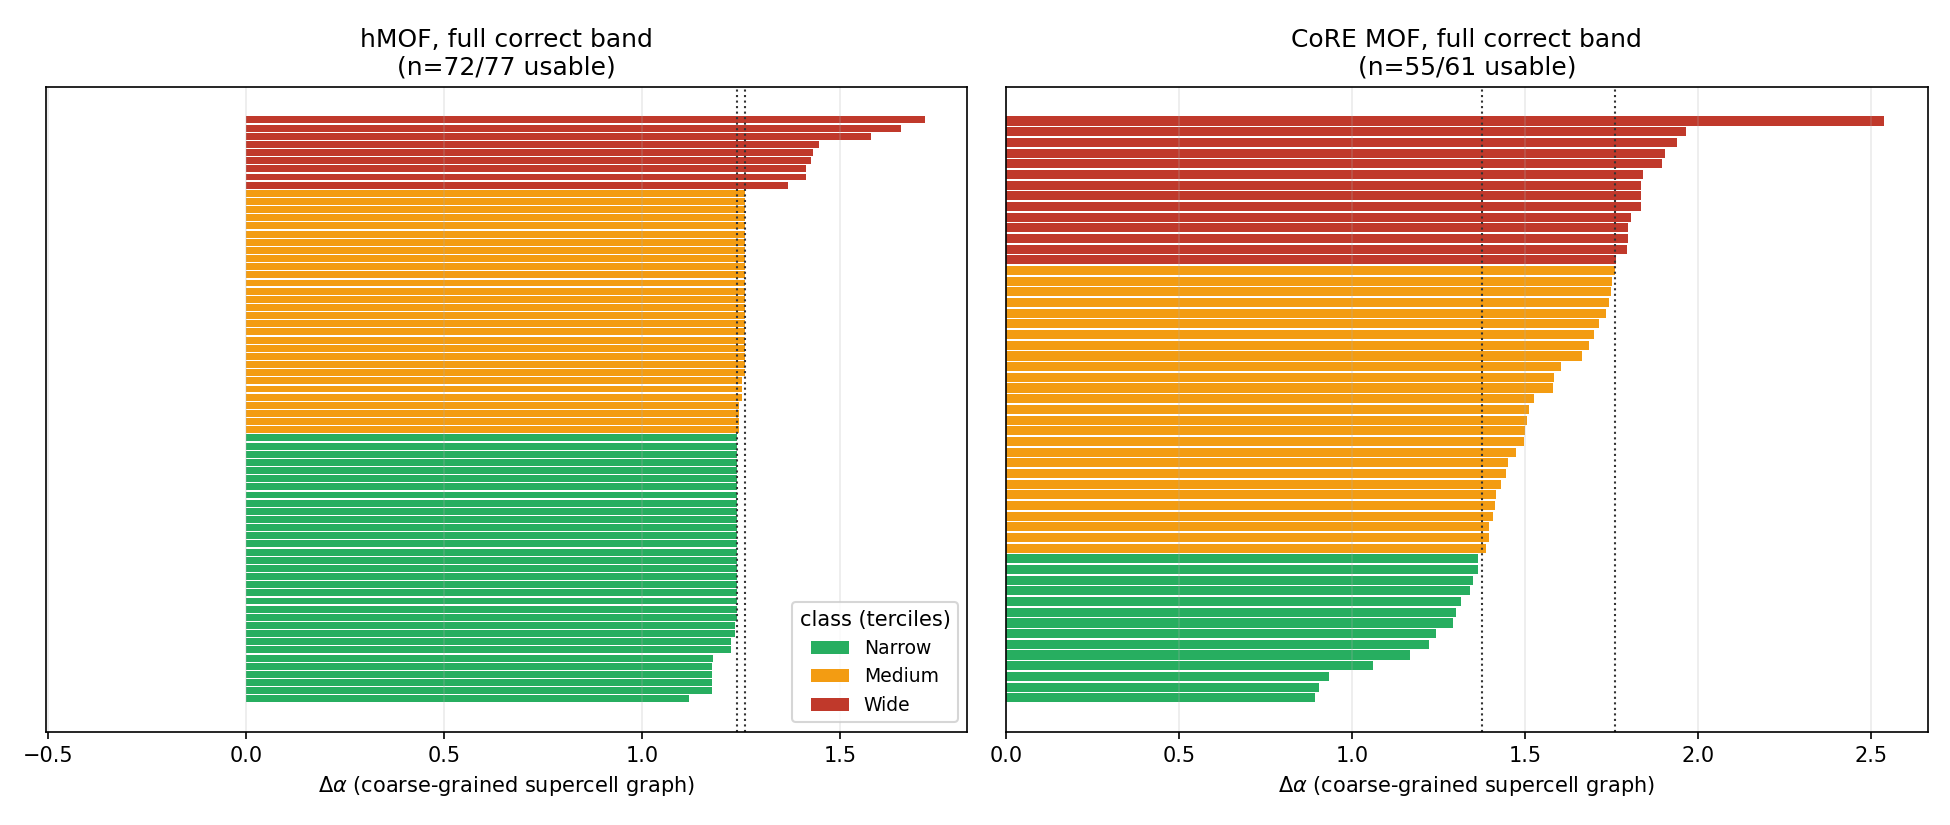
\includegraphics[width=0.99\linewidth,height=0.60\textheight,keepaspectratio]{fig15_full_band.png}%
}{%
  \fbox{\begin{minipage}{10cm}\centering\vspace{2cm}
  \textbf{[fig15\_full\_band.png]}\vspace{2cm}\end{minipage}}
}

\vspace{0.1cm}
{\scriptsize \textbf{What this shows.} Every structure in both complete datasets, on the
correct coarse-grained supercell graph --- not a sample, not the withdrawn atomic-graph
run --- sorted by $\Delta\alpha$ and coloured by its Narrow/Medium/Wide tercile. 72/77 hMOF
and 55/61 CoRE MOF produced a usable spectrum. \textbf{Purpose:} a single glance at whether
the band is one smooth spread or has visible structure worth explaining next.}
\end{frame}

% ---- the correlation evidence: does class track chemistry or graph size? ----
\begin{frame}{3d. Does Class Track Chemistry, or Graph Size?}
\framesubtitle{Why this graph: plots the one relationship the whole claim depends on, directly}
\centering
\IfFileExists{fig16_full_band_vs_size.png}{%
  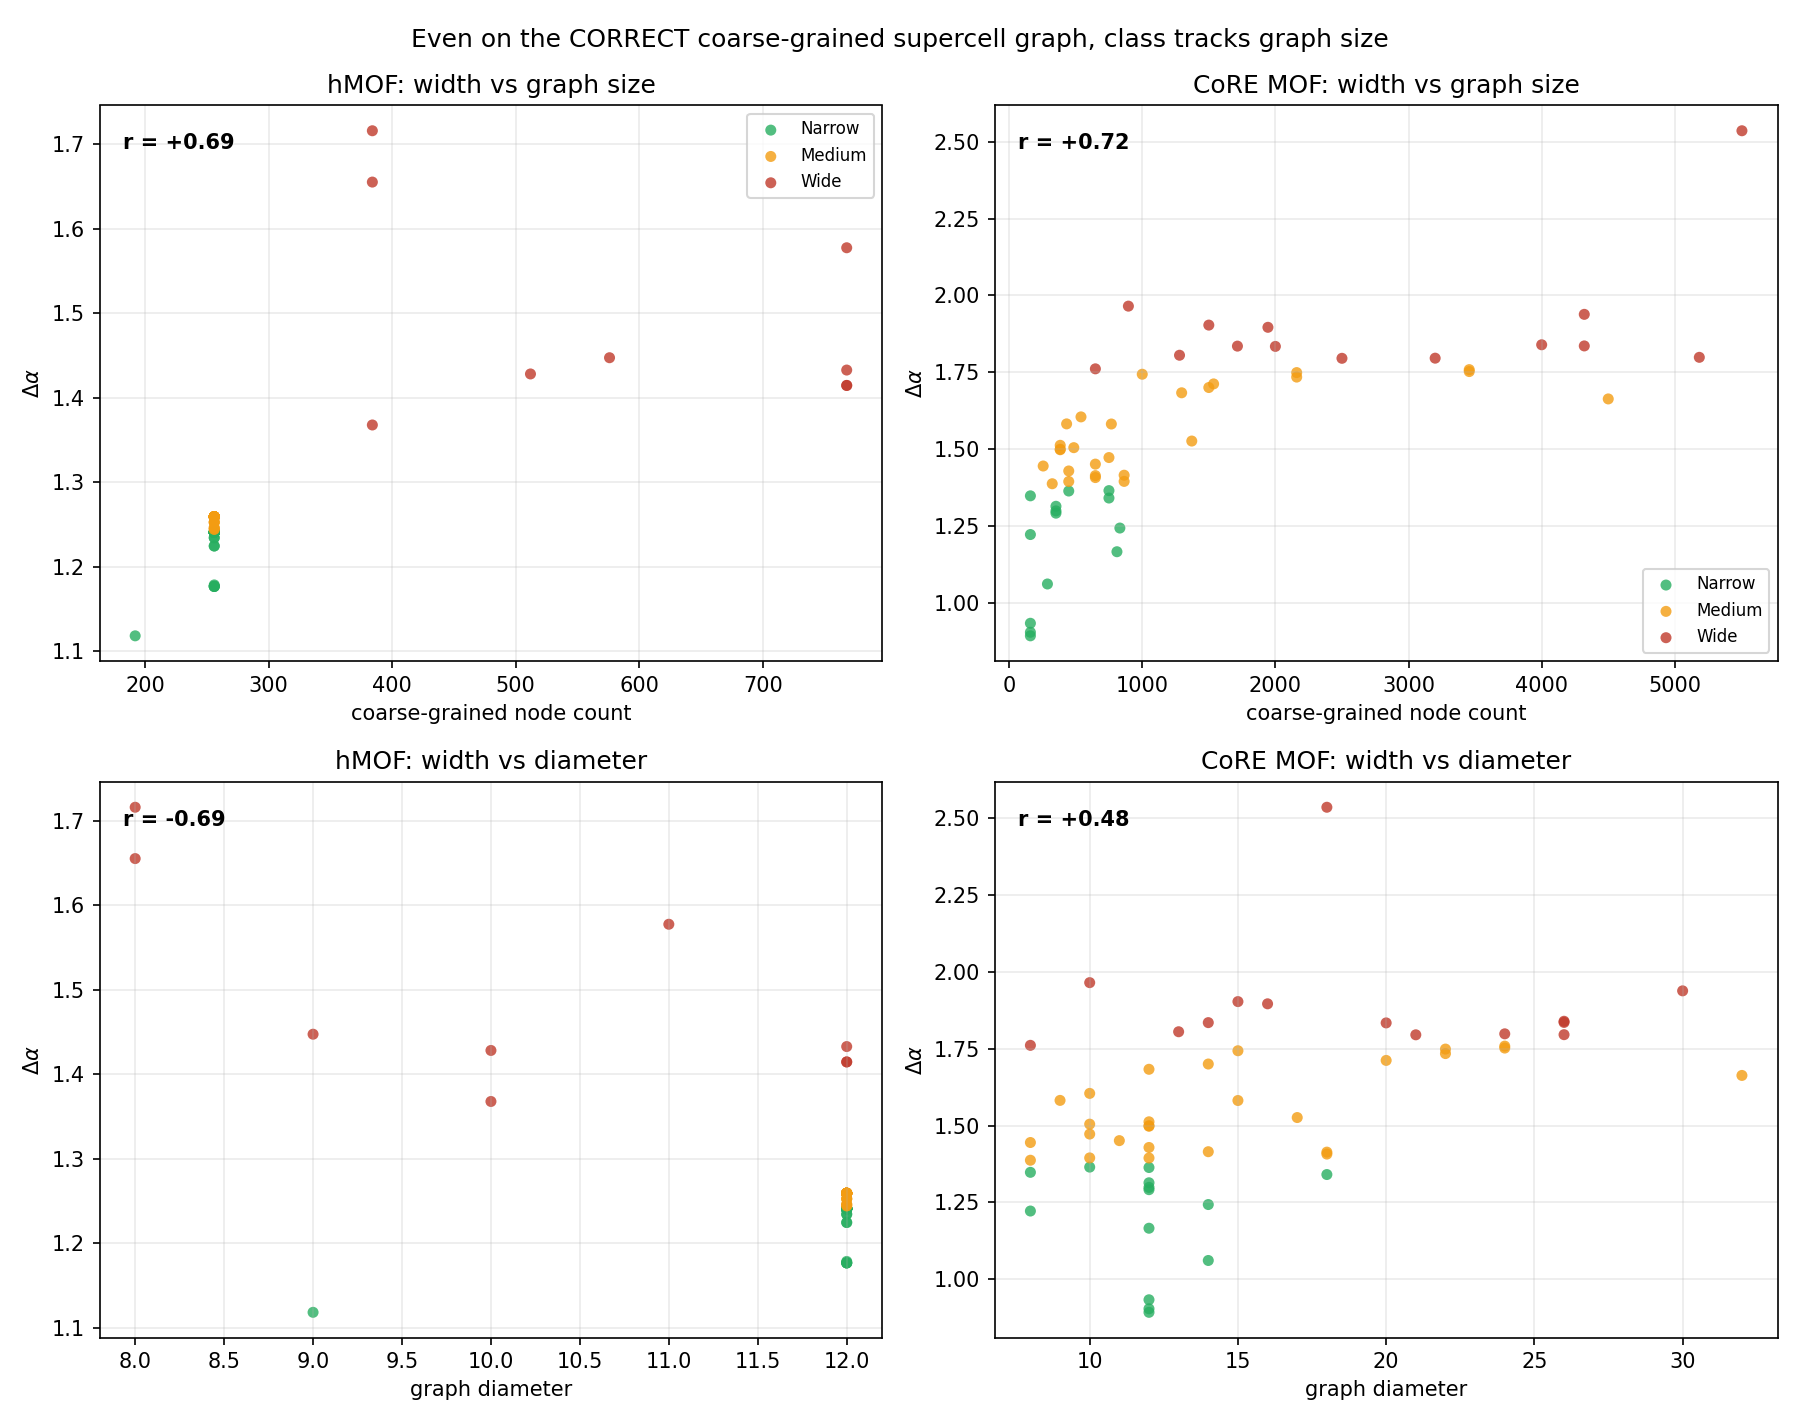
\includegraphics[width=0.99\linewidth,height=0.60\textheight,keepaspectratio]{fig16_full_band_vs_size.png}%
}{%
  \fbox{\begin{minipage}{10cm}\centering\vspace{2cm}
  \textbf{[fig16\_full\_band\_vs\_size.png]}\vspace{2cm}\end{minipage}}
}

\vspace{0.1cm}
{\scriptsize \textbf{What this shows.} $\Delta\alpha$ plotted directly against coarse-grained
node count and against graph diameter, both datasets, coloured by class. \textbf{Purpose:} if
class were chemistry, points would scatter freely against size; if class is standing in for
size, they will line up. They line up: $r=\mathbf{+0.69}$ (hMOF) and $r=\mathbf{+0.72}$
(CoRE MOF) against node count, independently, on the complete real dataset. \textbf{Using the
right graph fixes the graph. It does not fix the descriptor.}}
\end{frame}

% ---- our own spectra, both datasets, every curve ----
\begin{frame}{3e. Every Spectrum, Both Our Datasets}
\framesubtitle{Why this graph: a single Delta-alpha number hides shape --- this shows whether a whole class shares one}
\centering
\IfFileExists{fig17_grouped_spectra.png}{%
  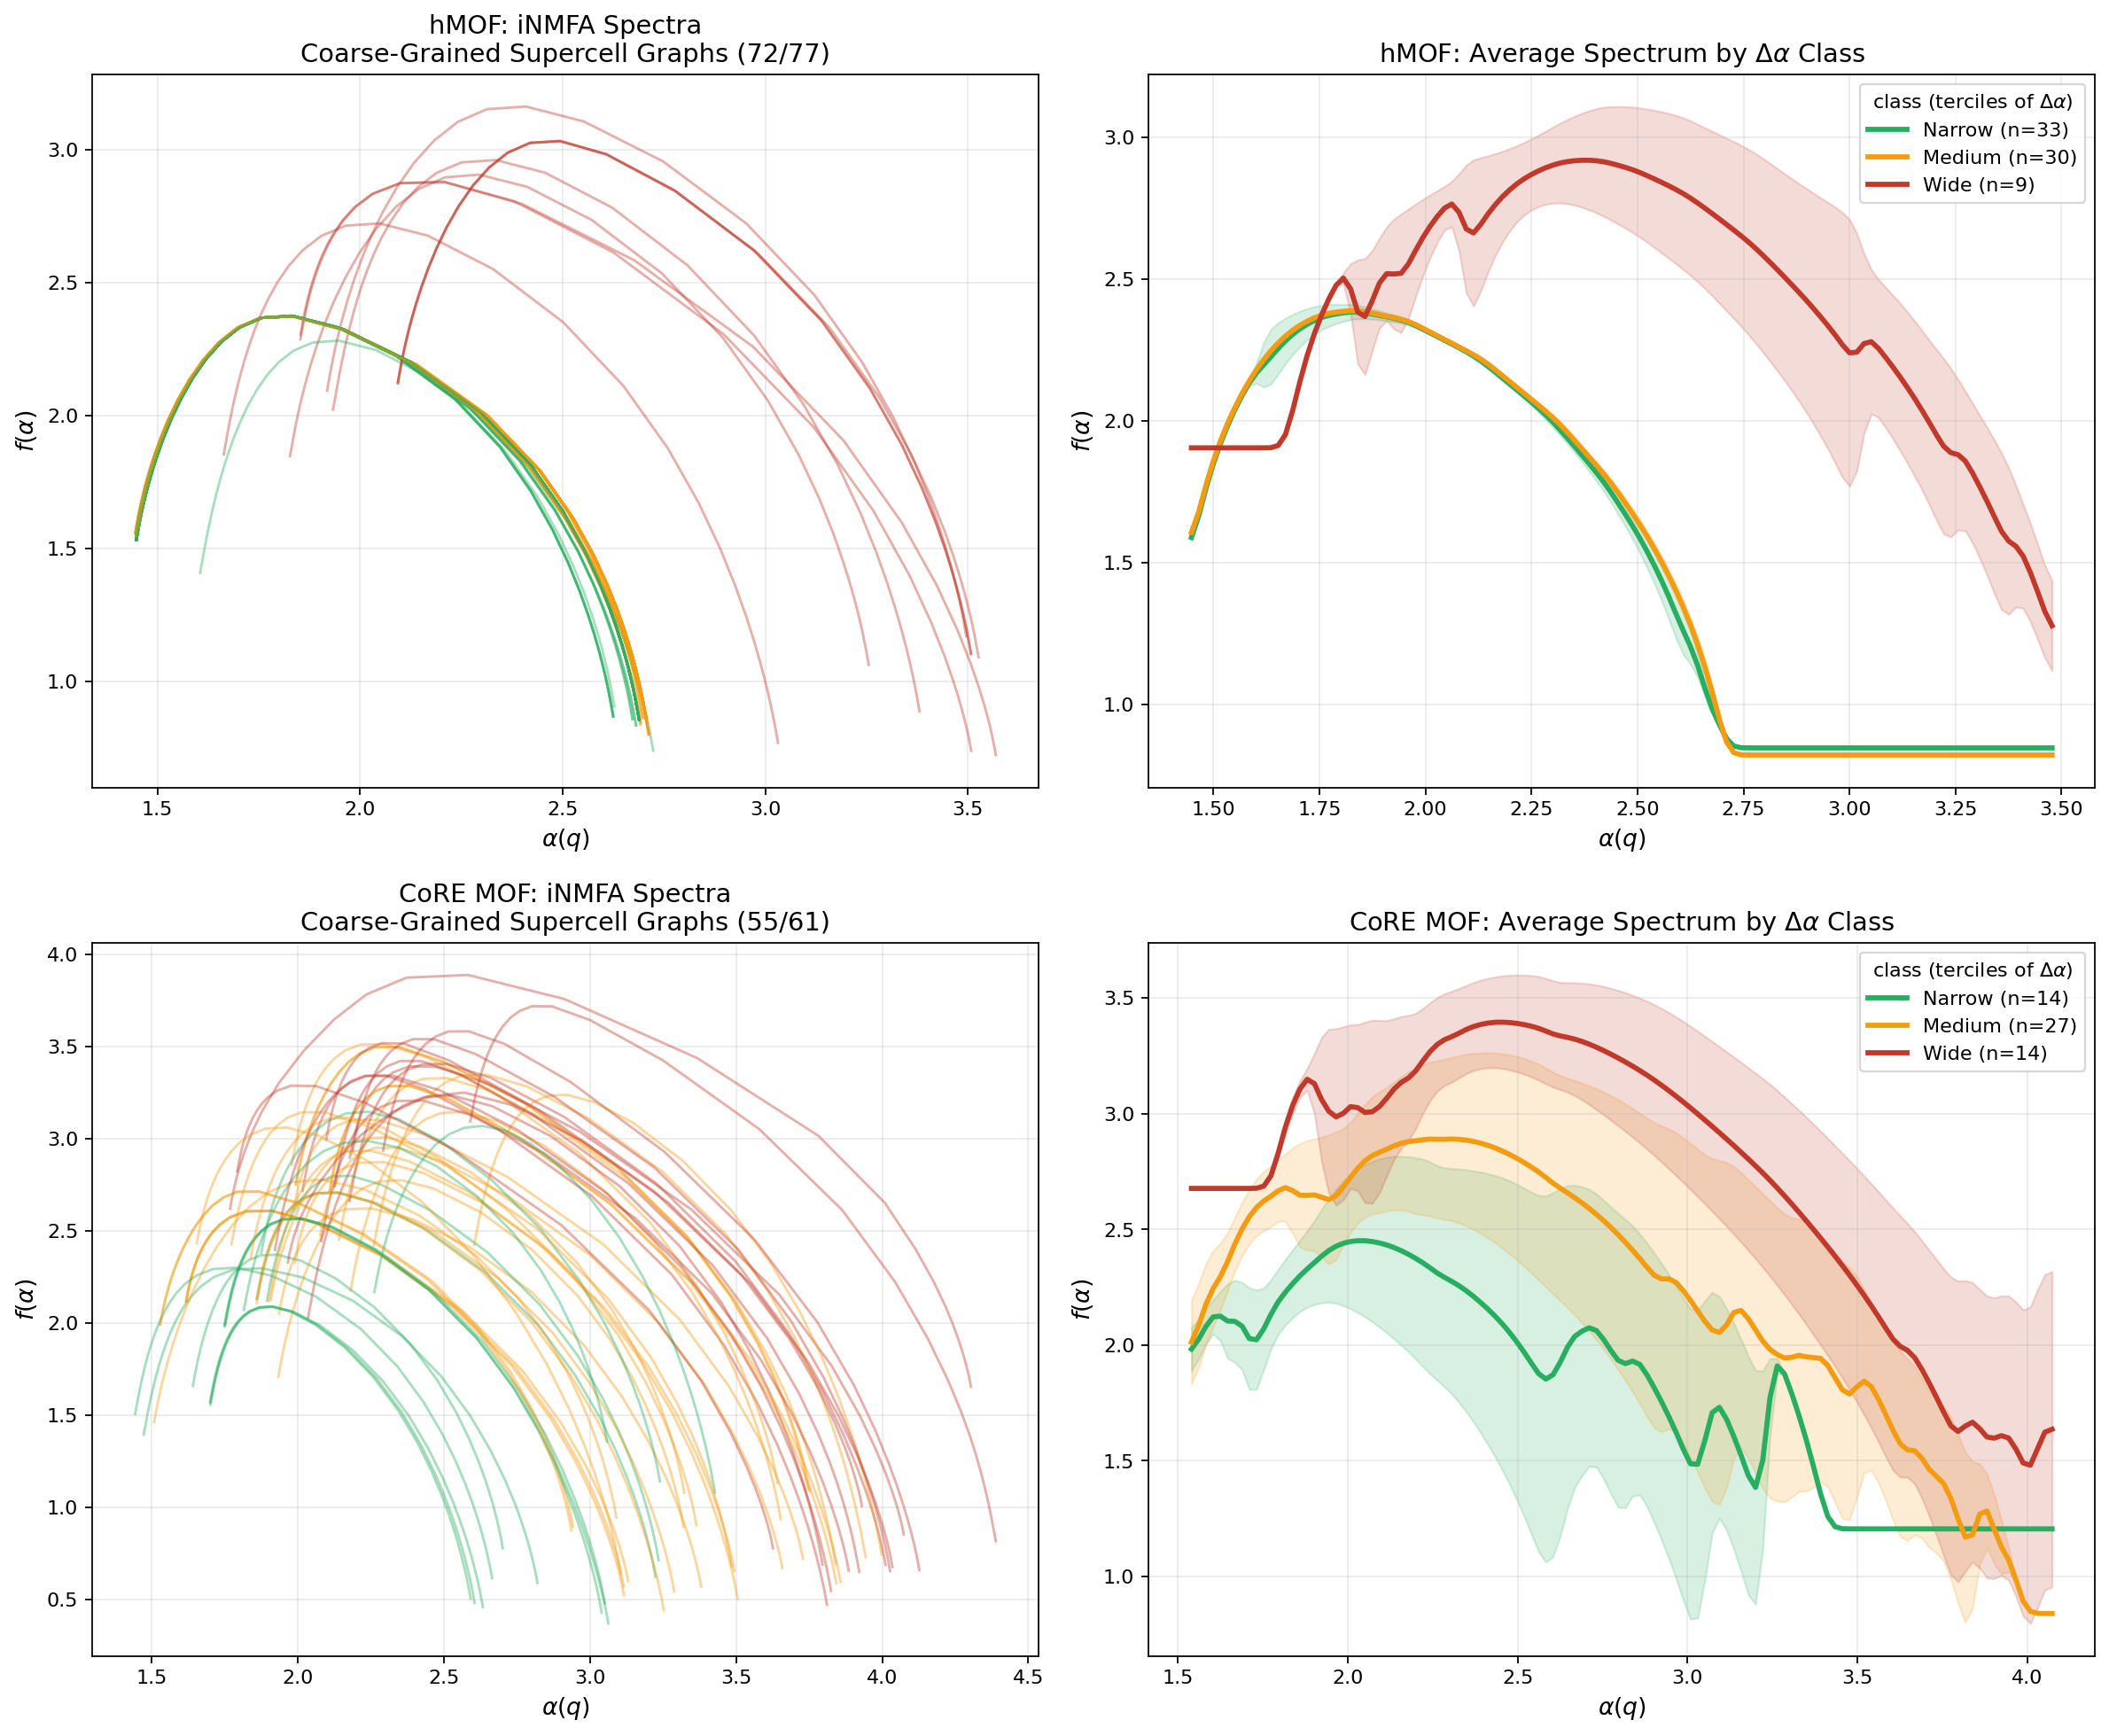
\includegraphics[width=0.88\linewidth,height=0.66\textheight,keepaspectratio]{fig17_grouped_spectra.png}%
}{%
  \fbox{\begin{minipage}{10cm}\centering\vspace{2cm}
  \textbf{[fig17\_grouped\_spectra.png]}\vspace{2cm}\end{minipage}}
}

\vspace{0.05cm}
{\scriptsize \textbf{What this shows.} Rows: hMOF, then CoRE MOF. Left column: every
individual spectrum, coloured by class. Right column: each class collapsed to its mean
$\pm$1 sd band. \textbf{Purpose:} answers whether an entire class traces one curve, or only
shares a similar width by coincidence --- the Wide (red) band sits visibly to the right of
and above the Narrow (green) band in both rows, meaning the whole spectrum shifts with class,
not just its width.}
\end{frame}

% ---- reference figures from an independent run, for direct comparison ----
\begin{frame}{3f. The Same Plotting Convention, an Independent Reference}
\framesubtitle{A separate coarse-grained run on CoRE MOF 2019 filtered to xenon-tested records}
\centering
\IfFileExists{fig17b_xenon_core_raw_reference.png}{%
  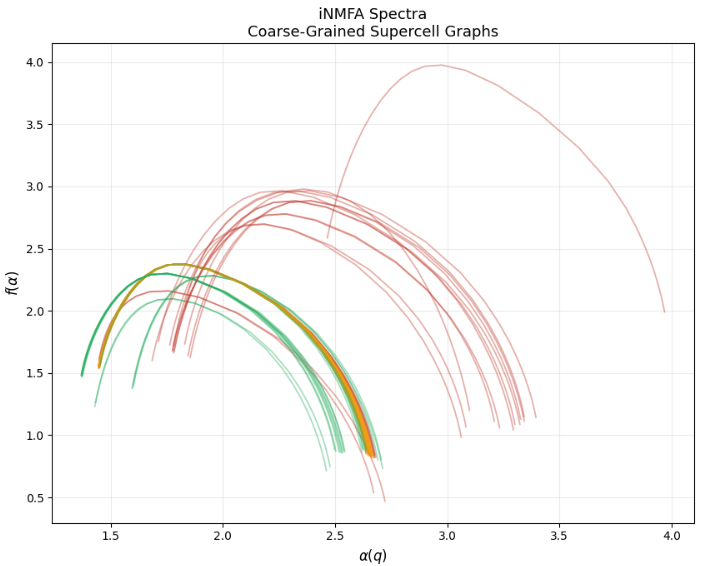
\includegraphics[width=0.48\linewidth,height=0.56\textheight,keepaspectratio]{fig17b_xenon_core_raw_reference.png}%
}{\fbox{\begin{minipage}{6cm}\centering\vspace{1.5cm}\textbf{[fig17b]}\vspace{1.5cm}\end{minipage}}}%
\hfill
\IfFileExists{fig17c_xenon_core_bands_reference.png}{%
  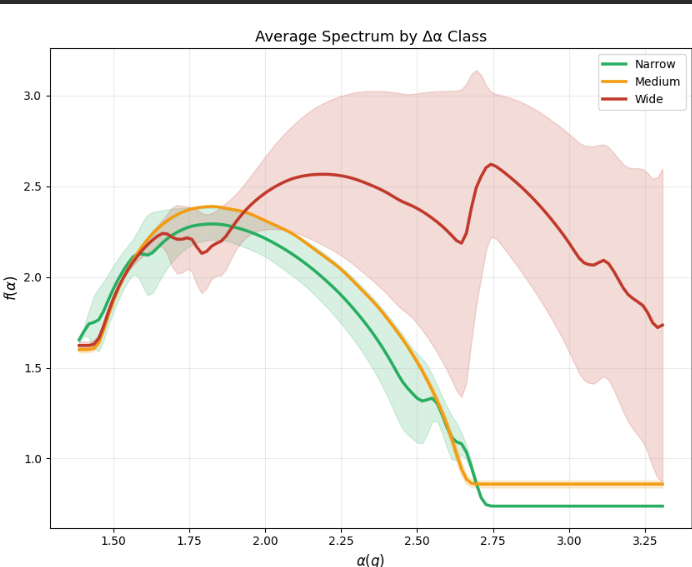
\includegraphics[width=0.48\linewidth,height=0.56\textheight,keepaspectratio]{fig17c_xenon_core_bands_reference.png}%
}{\fbox{\begin{minipage}{6cm}\centering\vspace{1.5cm}\textbf{[fig17c]}\vspace{1.5cm}\end{minipage}}}%

\vspace{0.1cm}
{\scriptsize \textbf{What this shows.} Reference figures, reproduced as-is, from an
independent coarse-grained run on \textbf{CoRE MOF 2019 filtered to xenon-tested records} ---
``xenon-tested'' names which gas-uptake simulation that database record carries, not an
element of the framework itself. Our own hMOF set is single-metal (Zn); our CoRE MOF set's
metal is unknown here (MOFX-DB supplied no MOFid for it). \textbf{Purpose:} the plotting
convention in 3e (raw spectra, then a smoothed class-average band) is shared with this
reference; the curves are not and should not be, since a different structure population
produced them. Shown for direct visual comparison, not as our own result.}
\end{frame}

% ============================ SLIDE 4: NEXT STEPS ============================
\section{Next Steps}
\begin{frame}{4. Remaining Work \& Timeline}
\framesubtitle{What is settled, what is still open, and what happens next}
\vspace{-0.3cm}
\begin{columns}[T]
\column{0.55\textwidth}
{\scriptsize
\setlength{\itemsep}{0pt}\setlength{\parskip}{1pt}
\textbf{Settled, and closed} \hfill \textcolor{okGreen}{\textbf{answered}}
\begin{itemize}\scriptsize
  \item \textbf{Which graph:} coarse-grained supercell, built by decomposing the unit cell
        first and replicating that small block graph --- proven identical to the reverse
        order, at a fraction of the cost (Slide 3).
  \item \textbf{Does the correct graph rescue the descriptor:} no, on the complete real
        dataset, checked directly (Slide 3d).
\end{itemize}

\textbf{Priority 1 --- Fix or retire $\Delta\alpha$} \hfill \textcolor{warnRed}{\textbf{now blocking}}
\begin{itemize}\scriptsize
  \item \textbf{Option A:} a size-independent redefinition. A fixed \textit{a-priori} $q$
        range does \textbf{not} work, tested directly; a different partition-function
        normalisation might.
  \item \textbf{Option B:} report the $\Delta\alpha(D)$ growth \textbf{slope} instead of the
        width, since the slope is well-defined even where the width is not. A capped check
        found the slope varies more across CoRE MOF than hMOF --- a candidate, stated as a
        proposal, not a result.
\end{itemize}

\textbf{Priority 2 --- Validate against measured properties} \hfill \textcolor{warnRed}{\textbf{blocked on Priority 1}}
\begin{itemize}\scriptsize
  \item Regressing a non-convergent number against real adsorption data would not be a
        meaningful test. This has to wait for Priority 1.
\end{itemize}
}
\column{0.45\textwidth}
\begin{block}{\footnotesize Position of the work, in one place}
\scriptsize
The \textbf{machinery is complete and verified}: decomposition, periodic graph, centrality
and the spectrum mathematics all work, cross-validated across two independent
implementations, on the complete 138-framework dataset, with 9 automated test suites gating
every push.

\vspace{0.08cm}
\textbf{Engineering $\approx$88\%. Scientific validation $\approx$35\%}, because the
headline descriptor does not converge with supercell size on any graph tested.
\textbf{Overall $\approx$55\%}, treating validation as a gate rather than averaging it away
with engineering --- reported this way on purpose.
\end{block}
\begin{block}{\footnotesize What would change this assessment}
\scriptsize
A size-independent definition of $\Delta\alpha$ (Priority 1) that still separates real
frameworks would move validation and the overall number together. Nothing short of that
does --- more structures, more test suites or a nicer platform would raise engineering
only, which is why the two percentages are kept separate rather than blended into one.
\end{block}
\end{columns}
\end{frame}

% ============================ REFERENCES =====================================
\section{References}
\begin{frame}{References (1 of 2)}
\framesubtitle{Every entry is a source the project actually uses}
{\tiny
\begin{itemize}\itemsep2pt
\item[{[1]}] B. J. Bucior \textit{et al.}, ``Identification Schemes for Metal--Organic Frameworks
      to Enable Rapid Search and Cheminformatics Analysis,'' \textit{Cryst. Growth Des.},
      19(11), 6682--6697, 2019. \hfill \textcolor{coolBlue}{\textbf{the decomposition we visualise}}
\item[{[2]}] J. Xiao, B. Wang, X. Li, ``Deciphering the Generating Rules and Functionalities of
      Complex Networks,'' \textit{Sci. Rep.}, 11, 22964, 2021.
      \hfill \textcolor{coolBlue}{\textbf{the method we implement}}
\item[{[3]}] C. Song, S. Havlin, H. A. Makse, ``Self-Similarity of Complex Networks,''
      \textit{Nature}, 433, 392--395, 2005.
\item[{[4]}] O. Delgado-Friedrichs, M. O'Keeffe, ``Identification of and Symmetry Computation
      for Crystal Nets,'' \textit{Acta Cryst. A}, 59(4), 351--360, 2003. \hfill (Systre)
\item[{[5]}] M. O'Keeffe \textit{et al.}, ``The Reticular Chemistry Structure Resource (RCSR),''
      \textit{Acc. Chem. Res.}, 41(12), 1782--1789, 2008. \hfill (net symbols)
\item[{[6]}] M. Eddaoudi \textit{et al.}, ``Modular Chemistry: Secondary Building Units\ldots,''
      \textit{Acc. Chem. Res.}, 34(4), 319--330, 2001. \hfill (the SBU concept)
\item[{[7]}] N. S. Bobbitt, J. Chen, R. Q. Snurr, ``MOFX-DB,'' \textit{J. Chem. Eng. Data},
      68(2), 483--498, 2023. \hfill \textcolor{coolBlue}{\textbf{our data source}}
\item[{[8]}] C. E. Wilmer \textit{et al.}, ``Large-Scale Screening of Hypothetical MOFs,''
      \textit{Nature Chem.}, 4(2), 83--89, 2012.
      \hfill \textcolor{warnRed}{\textbf{our 77 are hMOF = hypothetical}}
\item[{[9]}] Y. G. Chung \textit{et al.}, ``CoRE MOF 2019,'' \textit{J. Chem. Eng. Data},
      64(12), 5985--5998, 2019. \hfill \textcolor{warnRed}{\textbf{the set we still need}}
\item[{[10]}] B. Cordero \textit{et al.}, ``Covalent Radii Revisited,'' \textit{Dalton Trans.},
      2832--2838, 2008. \hfill (bond-perception cutoffs)
\end{itemize}}
\end{frame}

\begin{frame}{References (2 of 2)}
\framesubtitle{The four demonstration structures, and the tools used to build and check the graph}
{\tiny
\begin{itemize}\itemsep2pt
\item[{[11]}] S. S.-Y. Chui \textit{et al.}, \textit{Science}, 283, 1148--1150, 1999.
      \hfill (HKUST-1 --- test structure)
\item[{[12]}] H. Li, M. Eddaoudi, M. O'Keeffe, O. M. Yaghi, \textit{Nature}, 402, 276--279, 1999.
      \hfill (MOF-5 / IRMOF-1)
\item[{[13]}] K. S. Park \textit{et al.}, \textit{PNAS}, 103(27), 10186--10191, 2006.
      \hfill (ZIF-8 --- our chemical control)
\item[{[14]}] J. H. Cavka \textit{et al.}, \textit{JACS}, 130(42), 13850--13851, 2008.
      \hfill \textcolor{coolBlue}{\textbf{UiO-66 --- the 12-connected test}}
\item[{[15]}] G. C. Shearer \textit{et al.}, ``Defect Engineering: Tuning the Porosity and
      Composition of UiO-66,'' \textit{Chem. Mater.}, 28(11), 3749--3761, 2016.
      \hfill \textcolor{coolBlue}{\textbf{defects are real chemistry}}
\item[{[16]}] M. Fiedler, ``Algebraic Connectivity of Graphs,'' \textit{Czech. Math. J.},
      23(2), 298--305, 1973. \hfill ($\lambda_2$)
\item[{[17]}] U. Brandes, ``A Faster Algorithm for Betweenness Centrality,''
      \textit{J. Math. Sociol.}, 25(2), 163--177, 2001.
\item[{[18]}] A. H. Larsen \textit{et al.}, ``The Atomic Simulation Environment,''
      \textit{J. Phys. Condens. Matter}, 29(27), 273002, 2017. \hfill (ASE)
\item[{[19]}] A. A. Hagberg, D. A. Schult, P. J. Swart, ``Exploring Network Structure\ldots
      using NetworkX,'' \textit{SciPy2008}, 11--15. \hfill (NetworkX)
\end{itemize}}
\vspace{0.15cm}
{\scriptsize Full annotated list --- what each reference is \textit{for} --- in
\texttt{6\_references/README.md}.}
\end{frame}

% ============================ THANK YOU ======================================
\begin{frame}
\centering
{\Huge \textbf{\textcolor{amritaMaroon}{Thank You}}}\\[0.6cm]
{\footnotesize Interactive platform, source code and full documentation:}\\
{\small \textbf{github.com/Radha-Krishna-19/fyp}}
\end{frame}

\end{document}
